\documentclass[12pt]{article}
\usepackage{amsmath}
\usepackage{amsfonts}   % if you want the fonts
\usepackage{amssymb}    % if you want extra symbols
\usepackage{graphicx}   % need for figures
\usepackage{xcolor}
\usepackage{bm}
\usepackage{secdot}		
\usepackage{mathptmx}
\usepackage{float}
\usepackage[utf8]{inputenc}
\usepackage{textcomp}
\usepackage[hang,flushmargin,bottom]{footmisc} % footnote format

\usepackage{titlesec}
\titleformat{\section}{\normalsize\bfseries}{\thesection.}{1em}{}	% required for heading numbering style
\titleformat*{\subsection}{\normalsize\bfseries}

\usepackage{tocloft}	% change typeset, titles, and format list of appendices/figures/tables
\renewcommand{\cftdot}{}	
\renewcommand{\contentsname}{Table of Contents}
\renewcommand{\cftpartleader}{\cftdotfill{\cftdotsep}} % for parts
\renewcommand{\cftsecleader}{\cftdotfill{\cftdotsep}}
\renewcommand\cftbeforesecskip{\setlength{4pt}{}}
\addtolength{\cftfignumwidth}{1em}
\renewcommand{\cftfigpresnum}{\figurename\ }
\addtolength{\cfttabnumwidth}{1em}
\setlength{\tabcolsep}{35pt}


\usepackage[sorting=none]{biblatex}
\addbibresource{references.bib}


\usepackage{enumitem}         % to control spacing between bullets/numbered lists

\usepackage[hidelinks]{hyperref}
\hypersetup{
	colorlinks = true,
urlcolor ={blue},
citecolor = {.},
linkcolor = {.},
anchorcolor = {.},
filecolor = {.},
menucolor = {.},
runcolor = {.}
pdftitle={},
pdfsubject={},
pdfauthor={},
pdfkeywords={}
}
\urlstyle{same}

\usepackage{epstopdf} % converting EPS figure files to PDF

\usepackage{fancyhdr, lastpage}	% formatting document, calculating number of pages, formatting headers
\setlength{\topmargin}{-0.5in}
\setlength{\headheight}{40pt}
\setlength{\oddsidemargin}{0.25in}
\setlength{\evensidemargin}{0.25in}
\setlength{\textwidth}{6.0in}
\setlength{\textheight}{8.5in}

\usepackage{caption} % required for Figure labels
\captionsetup{font=small,labelfont=bf,figurename=Fig.,labelsep=period,justification=raggedright} 

\renewcommand\contentsname{Indice}


%   	BEGIN DOCUMENT 
%%%%%%%%%%%%%%%%%%%%%%%%%%%%%%%%%%%%%%%%%%%%%%%%%%%%%%%%%%%%%%%%%%%%
\begin{document}
	\urlstyle{rm} % Format style of \url   
%%%%%%%%%%%%%%%%%%%%%%%%%%%%%%%%%%%%%%%%%%%%%%%%%%%%%%%%%%%%%%%%%%%%
\begin{figure}[h!]
\vskip1in
\begin{center}

\includegraphics[scale = 2]{fig/logo.jpg}
\end{center}
\end{figure}

\begin{center}
\large{\textbf{Museum Informator}}
\end{center}

\vskip2.5cm

\begin{center}
a cura di
\end{center}

\vskip0.6cm

\begin{center}
\textbf{Pier Felice Balestrucci}\\
\textbf{Michele Lanotte}\\
\end{center}

\vskip3.5cm
 
\begin{center}
\textbf{Relazione del progetto di Modellazione Concettuale per il Web Semantico}
\end{center}

\begin{center}
\textbf{Università degli studi di Torino 2020/2021}
\end{center}
%%%%%%%%%%%%%%%%%%%%%%%%%%%%%%%%%%%%%%%%%%%%%%%%%%%%%%%%%%%%%%%%%%%%
%   Table of Contentsì
%%%%%%%%%%%%%%%%%%%%%%%%%%%%%%%%%%%%%%%%%%%%%%%%%%%%%%%%%%%%%%%%%%%%
\newpage
\begin{center}
\tableofcontents
\end{center}
\pagebreak
%%%%%%%%%%%%%%%%%%%%%%%%%%%%%%%%%%%%%%%%%%%%%%%%%%%%%%%%%%%%%%%%%%%%
\section{Motivazioni}
I musei rivestono un ruolo importante per ogni società: coinvolgono ed educano la comunità grazie alle parti di storia che raccontano, scandiscono il tempo e celano storie nascoste che si svelano durante la visione delle opere.  
Visitare un museo, lasciarsi ispirare da un’opera e trascorrere momenti in un luogo pieno di stimoli diventa una esperienza formativa oltre che educativa.

Nel periodo storico in cui stiamo vivendo, segnato dalla pandemia da covid19, i musei sono tra i pochi luoghi ancora accessibili sotto alcune strette restrizioni. Sviluppare un progetto che stimoli l’interesse di più persone risulta essere oltre che una sfida professionale anche sociale.
%%%%%%%%%%%%%%%%%%%%%%%%%%%%%%%%%%%%%%%%%%%%%%%%%%%%%%%%%%%%%%%%%%%%
\section{Requisiti}
L’obiettivo di questo progetto è creare innanzitutto uno strumento di consultazione. Infatti, seppur esistano numerosi siti web per i musei, questi risultano essere specifici di uno oppure di un insieme che ne condivide stesse caratteristiche (vicinanza geografica, temi, collezioni d’arte). 
L’idea ambiziosa è quella di raccogliere sotto uno stesso dominio il maggior numero di musei.

Accanto a questo obiettivo, ne sussiste un secondo. Si è voluto creare anche uno strumento che aiutasse a comporre itinerari turistici, indicando ad esempio i musei presenti in determinate città e che espongono certe collezioni artistiche.

Questa ontologia è pertanto orientata a diversi tipi di utenti, appassionati e non, che vogliono ottenere informazioni su determinate opere, artisti o musei, e a chi vuol sapere dove questi si trovino per comporre un percorso turistico che soddisfi le proprie curiosità.

Infine, a causa di questo periodo, essendoci limitazioni sugli spostamenti, sapere se ci sono monumenti o musei, specialmente all’aria aperta, da poter visitare nella propria città, può essere un’opportunità preziosa. Se ciò non fosse possibile però, molti musei organizzerebbero mostre virtuali per sopperire a tali mancanze.
%%%%%%%%%%%%%%%%%%%%%%%%%%%%%%%%%%%%%%%%%%%%%%%%%%%%%%%%%%%%%%%%%%%%
\newpage
\section{Descrizione del dominio}
Si definisce museo una raccolta pubblica o privata di opere relative all’arte, alla scienza e alla tecnica. La definizione di museo in Italia è quella data con il decreto del Presidente del Consiglio dei Ministri del 2 dicembre del 2019 che lo definisce “un’istituzione permanente, senza scopo di lucro, al servizio della società e del suo sviluppo. Aperto al pubblico compie ricerche che riguardano le testimonianze materiali e immateriali dell’umanità e del suo ambiente, le acquisisce, le conserva e, soprattutto le espone a fini di studio, educazione e diletto promuovendone la conoscenza presso il pubblico e la comunità scientifica.” \parencite{def1}

I musei sono un luogo di crescita interiore e professionale con un importante ruolo sociale. La Treccani, in particolare, descrive la funzione dei musei in relazione alla sfera umana: la crescita del desiderio di conoscenza, non più confinata tra ristrette schiere di privilegiati, ha fatto sì che i visitatori, sempre più spesso, cerchino nei musei non solo la conoscenza del passato, ma la possibilità di intravedere scenari futuri aderenti alle proprie intime speranze di sviluppo umano. \parencite{def2}

Le tipologie di musei sono molteplici e variano in base al numero e alla tipologia di opere che espongono, alle modalità di fruizione e alla posizione geografica (se si trovano in grandi o piccole città oppure in determinate parti del mondo).
Esemplificando le varie categorie, vi sono musei di arti figurative, di archeologia, di storia, di scienze naturali, zoologici eccetera.

Tra queste categorie, i musei d’arte sono sicuramente tra i più numerosi. Generalmente qui le opere vengono suddivise per periodi storici e scuola di provenienza: ad esempio, il museo del Louvre di Parigi presenta diverse collezioni come quella di arte antica, della scuola italiana e della scuola francese suddividendole per artisti e correnti alle quali appartengono. \parencite{louvre}

Infine, i musei ricoprono grande importanza soprattutto nel settore turistico veicolando flussi di persone in determinate città. Essi sono dei centri di raccolta che raccontano e riassumono la storia di un paese. Tra i musei più famosi e conosciuti ci sono il Museo del Louvre di Parigi e la Galleria degli Uffizi di Firenze, deterrenti importanti per il turismo in queste città.
%%%%%%%%%%%%%%%%%%%%%%%%%%%%%%%%%%%%%%%%%%%%%%%%%%%%%%%%%%%%%%%%%%%%
\newpage
\section{Documentazione}
La realizzazione di questo progetto ha visto innanzitutto lo studio di standard esistenti e l’esplorazione di vari siti web. Difatti esistono molte e diverse ontologie che trattano dei musei così come diversi siti che categorizzano le varie tipologie. 
Tra le varie ontologie prese in considerazione troviamo “Erlangen” del CIDOC Conceputal Reference Model (CRM) \parencite{cidoc}. Il CIDOC CRM è un tool teorico e pratico per l’integrazione dell’informazione nel campo dei beni culturali. Esso mira ad esplorare questioni complesse, guardando a diversi database e fornendo definizioni e strutture formali per descrivere concetti impliciti ed espliciti, generalmente d’interesse per l’argomento e usati nella documentazione del patrimonio culturale. Esso vuole fornire il “collante semantico” necessario per mediare tra diverse fonti di informazione sui beni culturali come quelle pubblicate da musei, biblioteche e archivi.
 Il CIDOC CRM si pone come uno standard progettato in modo da fornire sia il recupero di informazioni di alto livello che la formulazione e documentazione di dati specifici e di domande.
Un esempio della classe “Cose fatte dall’uomo” di questa ontologia è la seguente: 

\begin{figure}[!hb]
   \centering
   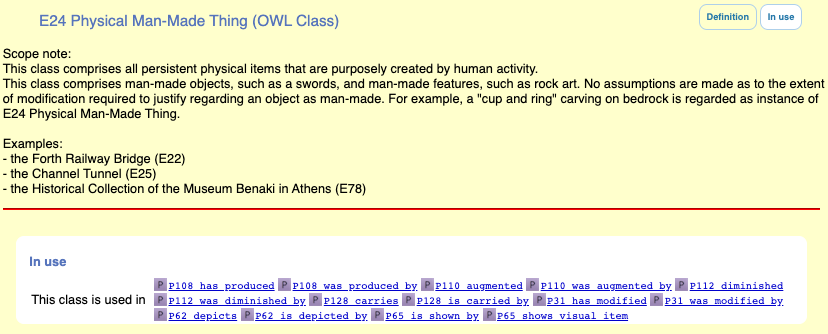
\includegraphics[scale=0.5]{fig/classe di CIDOC.png}
   \caption{Classe di Erlangen. Oggetti fisici fatti dall'uomo}\label{fig:picture}
\end{figure}

Una seconda ontologia esplorata è stata quella di Europeana che mira a caricare di significato i dati provenienti dal settore bibliotecario, museale, archivistico e audiovisivo costruendo uno stesso standard comune \parencite{europeana}. Più in particolare, essendo l’ambiente Linked Open Data mancante di dati autorevoli da parte della comunità dei beni culturali, l’Europeana Data Model (EDM) mira a colmare le varie lacune. 
\newpage
L’approccio adottato da Europeana si articola in vari punti:

\begin{itemize}
 \item EDM trascende gli standard dei metadati specifici del dominio, ma soddisfa la ricchezza di standard comunitari come LIDO per i musei 
 \item Facilita la partecipazione al web semantico
 \item Offre un modello di dati più sviluppato per offrire collegamenti più significati
 \item Questo approccio si traduce in una ricca scoperta di risorse e una visualizzazione migliore dei dati più complessi
\end{itemize} 
 
Infine, tra le varie ontologie preesistenti è stata rivolta attenzione anche a Core Ontology \parencite{core}, caso di studio realizzato dalla comunità italiana per il progetto europeo “Social Cohesion, Participation, And Inclusion Through Cultural Engagement”. Questa ricerca ha come obiettivo quello di consentire alle persone non udenti e ad altri visitatori di partecipare attivamente all’interpretazione culturale e allo storytelling e a connettersi e condividere interpretazioni attraverso le funzioni dei social media. Permettere, quindi, ai contributi di persone sorde di essere digitalmente accessibili a tutti nei musei ed online.

Dopo aver concluso la fase iniziale e aver pertanto scelto il dominio e formalizzato le finalità, si sono considerati diversi siti. Primo fra tutti Wikipedia, dove l’infobox di diverse entità ha permesso di porre le basi per la tassonomia dell’ontologia.
Di seguito viene mostrata la divisione dei musei in base alla loro tipologia \parencite{infomusei}.

\begin{figure}[!hb]
   \centering
   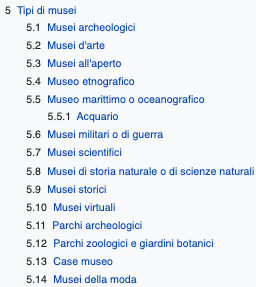
\includegraphics[scale=0.7]{fig/tassonomia musei wikipedia.png}
   \caption{Wikipedia Infobox musei}\label{fig:picture}
\end{figure}

Ai fini progettuali inoltre, è stata scelta la suddivisione delle varie opere in base alle discipline artistiche e, più in particolare, a quella che fa riferimento ai sensi umani. \parencite{infopere}

Per quanto riguarda l’istanziazione degli individui ci si è avvalsi di più siti web. Infatti, come specificato nell’introduzione, si è trovato difficile reperire siti con un insieme completo di individui consono agli obiettivi del progetto.
Tra questi, oltre alle singole pagine per monumenti e musei di Wikipedia, si riportano: 
\begin{itemize}
 \item \textbf{MUSEOItalia} che categorizza i musei italiani, li ripartisce per categorie e per comuni \parencite{museoitalia}
 \item \textbf{TheMet} che pone maggiore enfasi sulle collezioni d’arte \parencite{themet}
 \item \textbf{MoMAT} per colmare le mancanze di una ricerca poco fruttuosa sui musei orientali, in questo caso particolare giapponesi \parencite{momat}
\end{itemize} 

\begin{figure}[!h]
   \centering
   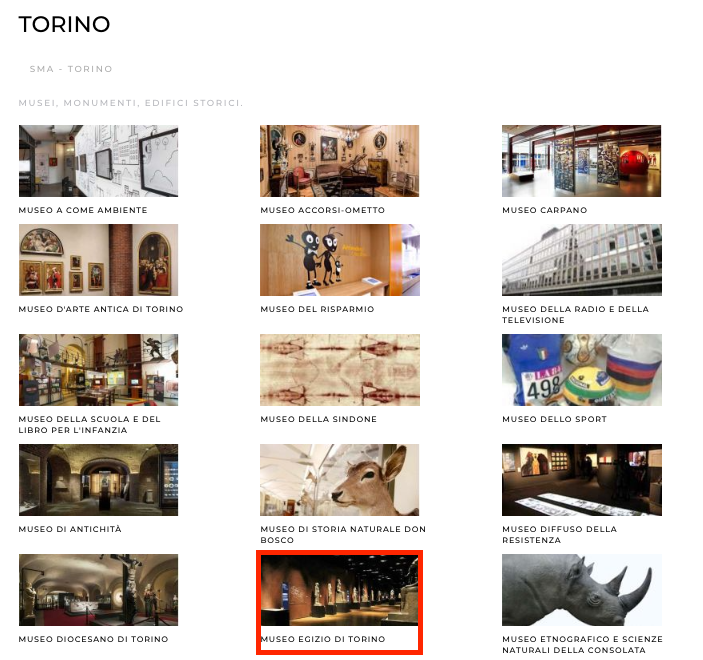
\includegraphics[scale=0.5]{fig/opera di MuseiITALIA.png}
   \caption{MUSEOItalia - Musei a Torino}\label{fig:picture}
\end{figure}
\begin{figure}[!h]
   \centering
   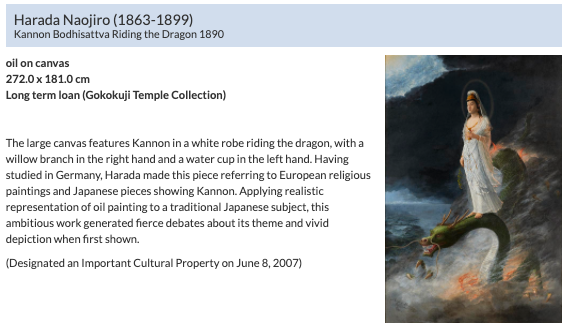
\includegraphics[scale=0.5]{fig/opera del Momat.png}
   \caption{Momat - Kannon Bodhissatva Rinding the Drago}\label{fig:picture}
\end{figure}

Infine, come già detto anticipatamente gli obiettivi di questo progetto sono anche quelli di creazione di uno strumento per comporre percorsi turistici. Di conseguenza si è ritenuto necessario inserire nella tassonomia dell’ontologia anche classi che si riferissero alle entità geografiche. Più in particolare, questa categorizzazione è stata pensata in modo più informale rispetto a quanto fatto finora scegliendo come ripartizione quella di città, nazione e continente. Accanto a questa classificazione, trova spazio l’introduzione di feature come quella del turismo cittadino e una classificazione di musei basata anche sul luogo in cui essi si trovano.

In conclusione, per ciò che concerne l’allineamento dell’ontologia con altri standard esistenti e design pattern, si riportano qui di seguito le classi importate delle prime:
\begin{itemize}
 \item \textbf{E71\_Human-Made\_Thing} $http://erlangen-crm.org/200717/E71_Human-Made\_Thing$:\\ comprende oggetti realizzati dall’uomo che sono documentati come unità singole. Questi oggetti sono prodotti intellettuali o oggetti fisici e sono caratterizzati da una relativa stabilità. Possono per esempio avere una forma fisica, un encoding elettrico o concetti o strutture logiche. Ad esempio il David di Michelangelo
 \item \textbf{Description} $https://w3id.org/italia/onto/l0/Description$:\\ Classe che si riferisce alle descrizioni delle opere. Ad esempio, il metodo usato per realizzarle.
\end{itemize} 
 
 Inoltre, sono state anche allineate le seguenti object properties hasDescription \\$https://w3id.org/italia/onto/l0/hasDescription$ e la sua inversa isDescriptionOf \\$https://w3id.org/italia/onto/l0/isDescriptionOf$ che rappresentano la descrizione di un’opera.

Per i design pattern si è scelto di implementare “Collection” \\$http://www.ontologydesignpatterns.org/cp/owl/collectionentity.owl\#Collection$ che rappresenta una collezione, in questo caso d'arte. Laddove essa è un insieme di opere rifacente a un periodo, una cultura, un'area geografica.
%%%%%%%%%%%%%%%%%%%%%%%%%%%%%%%%%%%%%%%%%%%%%%%%%%%%%%%%%%%%%%%%%%%%
\newpage
\section{Documentazione con LODE}
L’ontologia e le triple materializzate inferite sono state caricate in formato .owl e .ttl all'indirizzo Github: \href{https://github.com/ModSem20-21/MuseumOntology/tree/master/Ontologia}{ModSem20-21/MuseumOntology}.\\
Inoltre, tramite lo strumento LODE è stata creata una documentazione dell’ontologia consultabile a quest'altro \href{https://github.com/ModSem20-21/MuseumOntology/tree/master/Documentazione%20LODE}{indirizzo}. 
%%%%%%%%%%%%%%%%%%%%%%%%%%%%%%%%%%%%%%%%%%%%%%%%%%%%%%%%%%%%%%%%%%%%
\newpage
\section{Visualizzazione}
Una versione interattiva della tassonomia delle classi, generata tramite WebVOWL, è disponibile a questo indirizzo \href{http://www.visualdataweb.de/webvowl/#iri=https://raw.githubusercontent.com/ModSem20-21/MuseumOntology/master/Ontologia/MuseumInformator.owl}{qui}.\\
I template principali dell'ontologia sono relativi ai musei e alle opere (e quindi, gli artisti che le hanno realizzate).\\
Per questi sono riportati di seguito i grafici e le relative triple dell'esempio in forma tabellare.


\begin{figure}[H]
   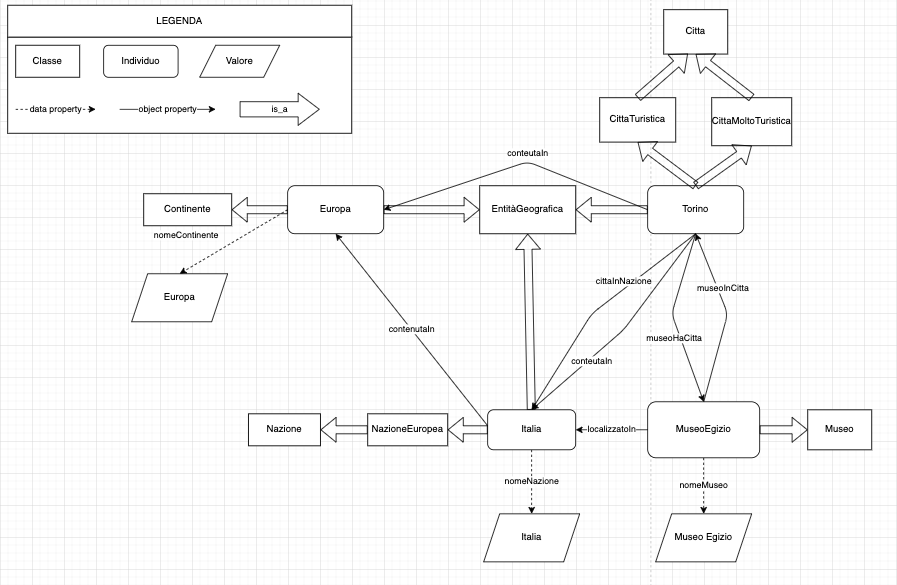
\includegraphics[scale=0.48]{fig/template Museo.png}
   \caption{Template dei musei}\label{fig:picture}
\end{figure}

Si precisa che il prefisso nelle tabelle ":" equivale a \\$<http://www.semanticweb.org/utente/ontologies/2020/11/MuseumOntology\#>$
\newline
\begin{center}
 \begin{tabular}{ |p{3cm}|p{3cm}|p{3cm}| }
 \hline
 \multicolumn{3}{|c|}{\textbf{Template Museo}} \\
 \hline
 \textbf{Soggetto} & \textbf{Predicato} & \textbf{Oggetto}\\
 \hline
 :MuseoEgizio & rdf:type &:Museo   \\
  \hline
 :MuseoEgizio &   :nomeMuseo  & “Museo Egizio”\textasciicircum \textasciicircum xsd:string   \\
  \hline
 :MuseoEgizio & :localizzatoIn & :Italia\\
  \hline
 :MuseoEgizio &:museoInCitta & :Torino\\
  \hline
 :Italia & rdf:type & :NazioneEuropea\\
  \hline
 :Italia & rdf:type  & :Nazione   \\
  \hline
 :Italia & rdf:type  & :EntitàGeografica\\
  \hline
 :Italia & :nomeNazione  & “Italia”\textasciicircum \textasciicircum xsd:string   \\
  \hline
 :Italia & :contenutaIn  & :Europa\\
  \hline
 :Europa & rdf:type  & :Continente   \\
  \hline
 :Europa & rdf:type  & :EntitàGeografica\\
  \hline
 :Europa & :nomeContinente  & “Europa” \textasciicircum \textasciicircum xsd:string\\
  \hline
 :Torino &   rdf:type  & :CittaTuristica\\
  \hline
 :Torino & rdf:type  & :CittaMoltoTuristica   \\
  \hline
 :Torino & rdf:type  & :Citta\\
  \hline
 :Torino & rdf:type  & :EntitàGeografica   \\
  \hline
 :Torino & :contenutaIn  & :Europa\\
  \hline
 :Torino &   :contenutaIn  & :Italia\\
  \hline
 :Torino &   :cittaInNazione  & :Italia\\
 \hline
\end{tabular}
\end{center}


\begin{figure}[H]
   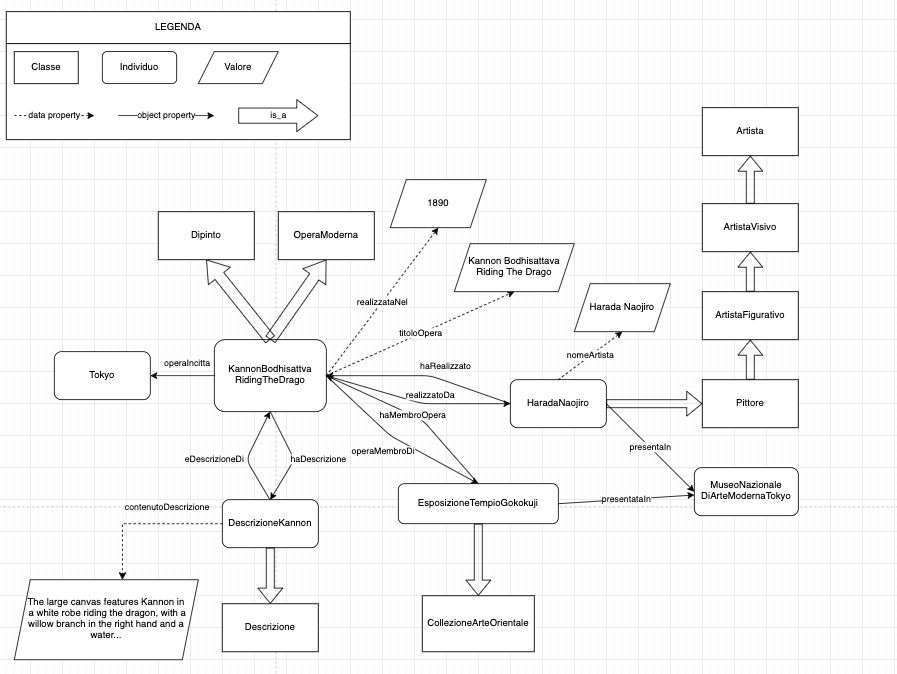
\includegraphics[scale=0.48]{fig/template Opera.png}
   \caption{Template per opere e artisti}\label{fig:picture}
\end{figure}

\begin{center}
 \begin{tabular}{ |p{3cm}|p{3cm}|p{3cm}| }
 \hline
 \multicolumn{3}{|c|}{\textbf{Template Opere e Musei}} \\
 \hline
 \textbf{Soggetto} & \textbf{Predicato} & \textbf{Oggetto}\\
 \hline
 :KannonBodhisattva RidingTheDrago & rdf:type & :Dipinto   \\
 \hline
 :KannonBodhisattva RidingTheDrago &   rdf:type  & :OperaModerna\\
  \hline
 :KannonBodhisattva RidingTheDrago & :operaInCitta & :Tokyo\\
  \hline
 :KannonBodhisattva RidingTheDrago &:haDescrizione & :DescrizioneKannon\\
  \hline
 :KannonBodhisattva RidingTheDrago & realizzataNel & "1890”\textasciicircum \textasciicircum xsd:unsignedInt\\
 \hline
 :KannonBodhisattva RidingTheDrago & :titoloOpera  & “Kannon Bodhisattava Riding The Drago”\textasciicircum \textasciicircum xsd:string  \\
 \hline
 :KannonBodhisattva RidingTheDrago & :realizzatoDa  & :HaradaNaojiro\\
 \hline
 :KannonBodhisattva RidingTheDrago & :operaMembroDi  & :Esposizione TempioGokokuji   \\
 \hline
 :DescrizioneKannon & rdf:type  & :Descrizione\\
 \hline
 :DescrizioneKannon & :contenutoDescrizione  & “The large canvas ...”\textasciicircum \textasciicircum xsd:string   \\
 \hline
 :DescrizioneKannon & :eDescrizioneDi  & :KannonBodhisattva RidingTheDrago\\
 \hline
 :Esposizione TempioGokokuji & rdf:type  & :Collezione ArteOrientale\\
 \hline
 :Esposizione TempioGokokuji & :haMembroOpera  & :KannonBodhisattva RidingTheDrago\\
 \hline
 :Esposizione TempioGokokuji & :presentataIn  & :MuseoNazionale DiArteModernaTokyo   \\
 \hline
 :HaradaNaojiro & rdf:type  & :Pittore\\
 \hline
 :HaradaNaojiro & rdf:type  & :ArtistaFigurativo   \\
 \hline
 :HaradaNaojiro & rdf:type  & :ArtistaVisivo\\
 \hline
 :HaradaNaojiro & rdf:type  & :Artista\\
 \hline
 :HaradaNaojiro & :presentaIn  & :MuseoNazionale DiArteModernaTokyo\\
 \hline
  :HaradaNaojiro & :nomeArtista  & “Harada Naojiro”\textasciicircum \textasciicircum xsd:string\\
  \hline
 :HaradaNaojiro & :haRealizzato  & :KannonBodhisattva RidingTheDrago\\
 \hline
\end{tabular}
\end{center}
%%%%%%%%%%%%%%%%%%%%%%%%%%%%%%%%%%%%%%%%%%%%%%%%%%%%%%%%%%%%%%%%%%%%
\newpage
\section{Queries SPARQL e Applicazione Client}
Nella progettazione del flusso di interazione con l’utente, e quindi delle query SPARQL, si è mantenuta costante attenzione sugli obiettivi del progetto. Difatti si voleva creare sia un sistema di consultazione sia di creazione di itinerari turistici. 
Una rappresentazione che mostra il risultato di questa fase è la seguente:
\begin{figure}[!h]
   \centering
   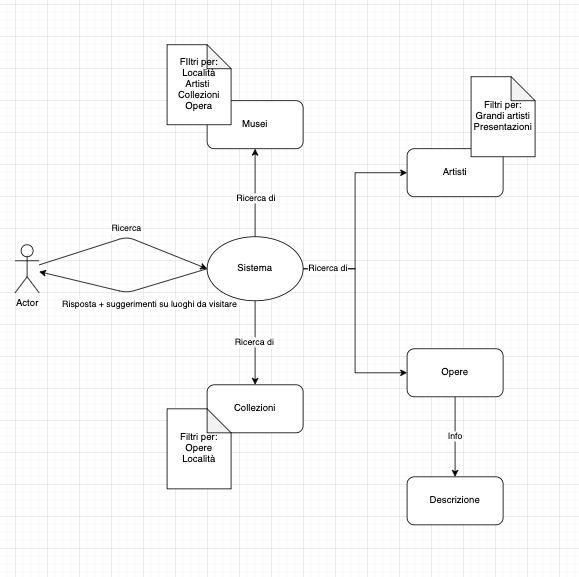
\includegraphics[scale=0.6]{fig/flowchart interazione.png}
   \caption{Flusso di interazione con l'utente}\label{fig:picture}
\end{figure}

L’utente, in questo caso “Actor” nella figura, può chiedere al sistema di ricercare musei, artisti, opere o collezioni e per ciascuna di queste categorie usare una serie di filtri per facilitarla. Inoltre, questi ultimi sono generalmente pensati proprio per offrire anche la località di ciò che si cerca. Di rilievo è sicuramente il sistema di suggerimenti proposto. Seppur questo non sia un progetto orientato alla profilazione utente, si è sfruttata la struttura dell’ontologia per dare suggerimenti “naive”. Infatti, il sistema consiglierà all’utente di visitare città particolarmente turistiche o artisti che hanno prodotto molte opere.

Il passo successivo è stato elaborare dei mockup che rendessero l'idea di ciò che sarebbe stata l'interazione.
\begin{figure}[!ht]
   \centering
   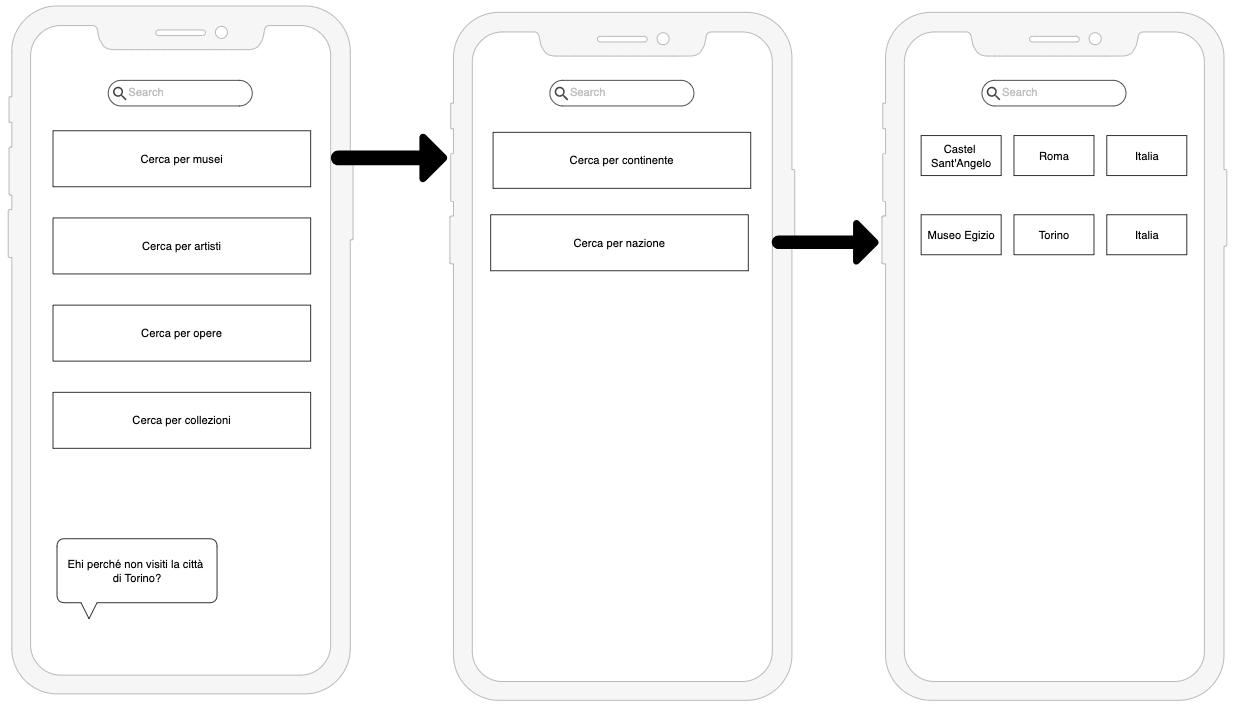
\includegraphics[scale=0.35]{fig/moqup1.png}
   \caption{Mockup - Interazione con "Musei"}\label{fig:picture}
\end{figure}
\begin{figure}[!ht]
   \centering
   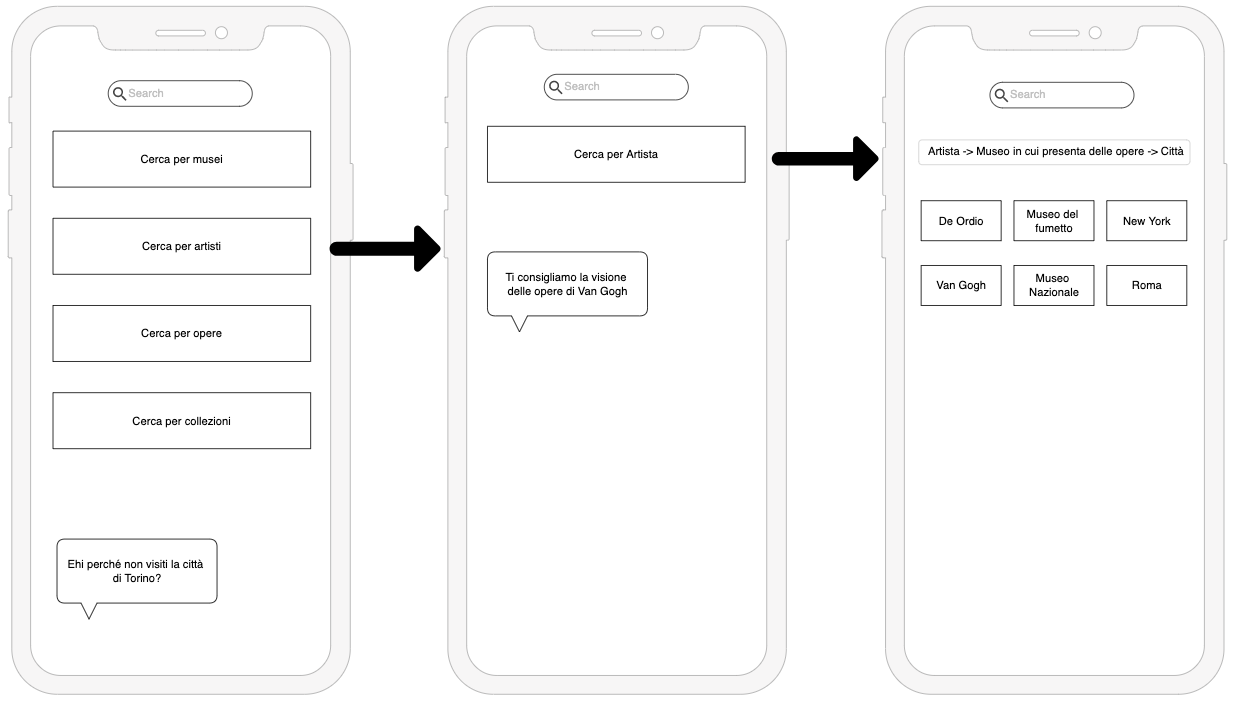
\includegraphics[scale=0.35]{fig/moqup2.png}
   \caption{Mockup - Interazione con "Artisti"}\label{fig:picture}
\end{figure}

L’applicazione client realizzata a partire dalla fase di progettazione verrà esaminata nelle successive pagine. Si noti che per ogni schermata vi è la query SPARQL realizzata a supporto dell’interazione. Ciò è stato reso possibile caricando l'ontologia inferita su Virtuoso e interrogando l'endpoint SPARQL messo a disposizione.

\begin{figure}[!ht]
   \centering
   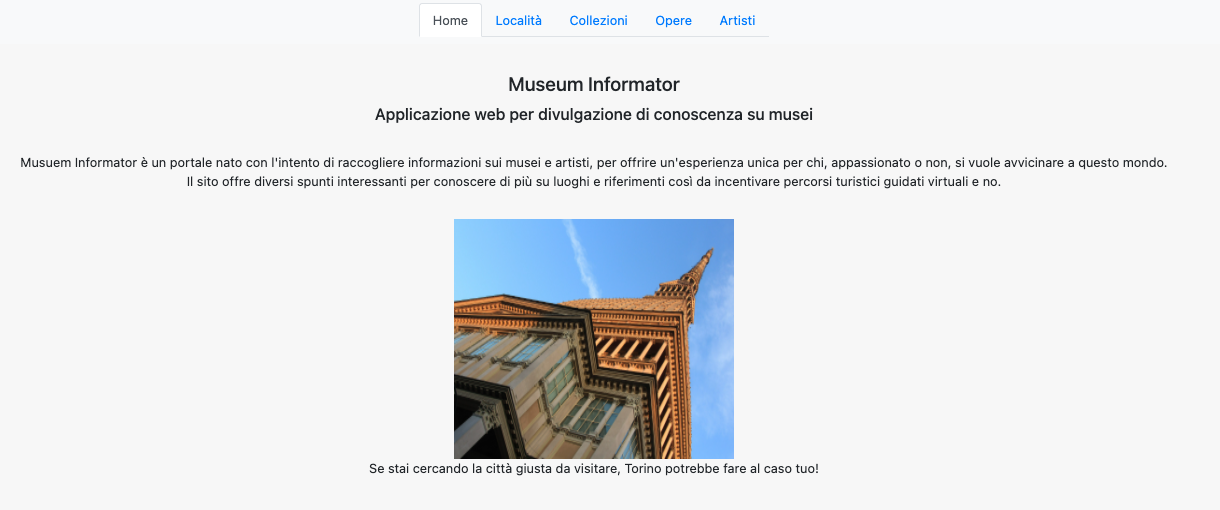
\includegraphics[scale=0.35]{fig/Schemata 1 webapp.png}
   \caption{Web App - Schermata di Home}\label{fig:picture}
\end{figure}

La prima schermata che viene mostrata è la homepage. Oltre a una breve descrizione che spiega le finalità dell’applicazione, il sistema offre da subito un suggerimento turistico, ossia una città da visitare.
L’ottenimento di questo risultato è dato dal congiungimento in via programmatica delle seguenti query:

\begin{itemize}
 \item SELECT (MAX(?count) as ?max) WHERE{ SELECT ?citta (count(*) as ?count) WHERE { ?museo museum:museoInCitta ?citta} GROUP BY ?citta}
 \item SELECT ?citta (count(*) as ?count) WHERE { ?museo museum:museoInCitta ?citta} GROUP BY ?citta
\end{itemize} 

Dove la prima query restituisce il numero di musei più grande tra tutte le città; mentre la seconda il numero di musei nelle varie città. Unendo questi due risultati, si è ricavato che Torino è la città più turistica. 
\\
\\
La seconda schermata, “Località” mostra i musei nei vari continenti, quindi nelle varie nazioni e città. L’utente può scegliere anche di filtrare in base alla località che preferisce. L’ottenimento di tale risultato è dato dall’unione anche in questo caso di due query: la prima che si riferisce alla nostra ontologia; la seconda fatta all’endpoint SPARQL di Wikidata.

\begin{figure}[!h]
   \centering
   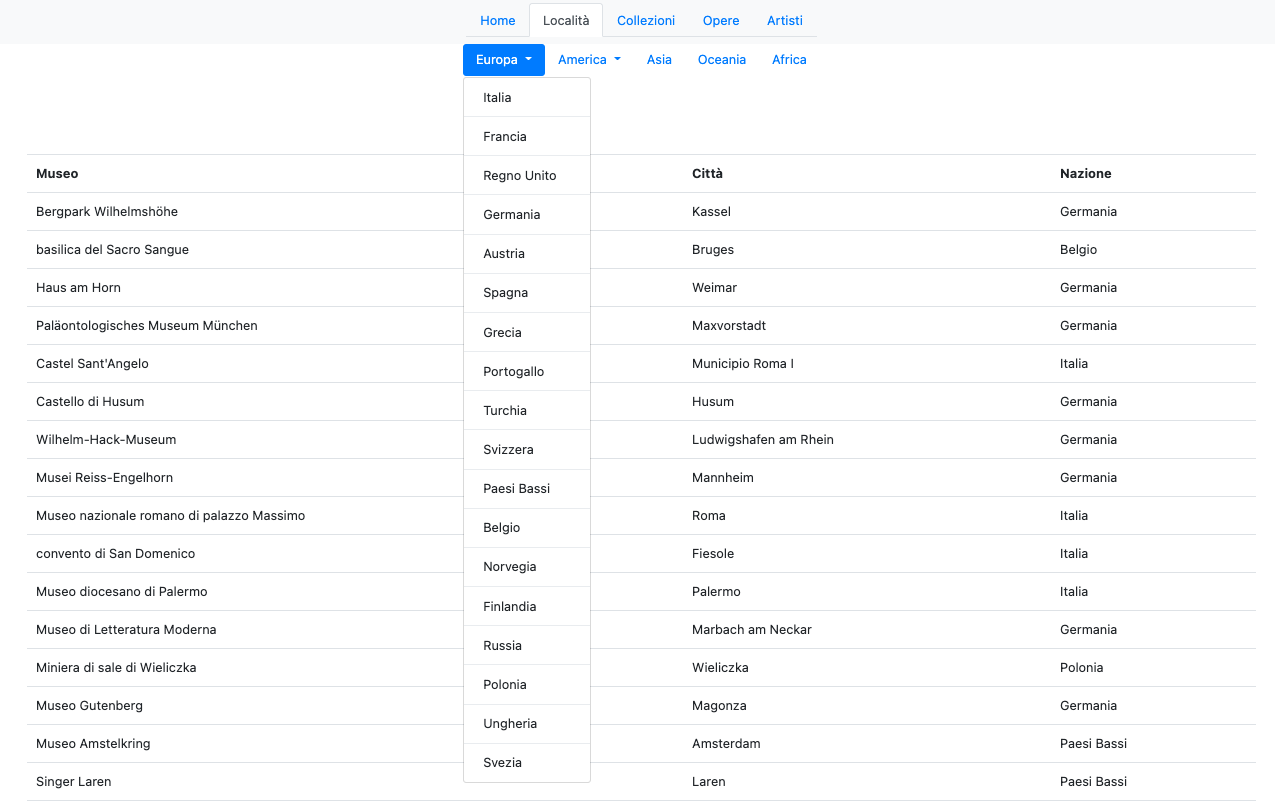
\includegraphics[scale=0.30]{fig/Schermata 2 webapp.png}
   \caption{Web App - Località}\label{fig:picture}
\end{figure}

\begin{itemize}
 \item SELECT ?museo ?citta ?nazione ?continente WHERE {?museo museum:museoInCitta ?citta. ?citta museum:contenutaIn ?nazione. ?nazione rdf:type museum:Nazione. ?nazione museum:contenutaIn ?continente} ORDER BY ?continente, ?nazione
 \item SELECT DISTINCT ?museoLabel ?PaeseLabel ?continenteLabel\\ ?unit\_\_amministrativa\_in\_cui\_\_\_situatoLabel WHERE { SERVICE wikibase:label\\ { bd:serviceParam wikibase:language "[AUTO\_LANGUAGE],it". } ?museo wdt:P31 wd:Q33506. ?museo wdt:P17 ?Paese. ?museo wdt:P131 ?unit\_\_amministrativa\_in\_cui\_\_\_situato. ?Paese wdt:P30 ?continente. } LIMIT 100
\end{itemize} 

La terza schermata mostra le varie collezioni che sono collocate nei musei o nelle città. Anche in questo caso l’utente per entrambe le scelte può filtrare, per l’appunto, per città e per musei.
Le query in ordine per schermata sono:
\begin{itemize}
 \item SELECT ?collezione ?citta WHERE {?collezione museum:presentataIn ?museo. ?museo museum:museoInCitta ?citta. FILTER regex(?citta, $<$city$>$)}
 \item SELECT ?collezione ?museo WHERE { ?collezione museum:presentataIn ?museo.  FILTER regex(?museo, $<$museum$>$).}
\end{itemize} 

Si noti come in entrambe le query è possibile effettuare il filtraggio in base a ciò che l’utente scrive nella barra di ricerca.

\begin{figure}[!h]
   \centering
   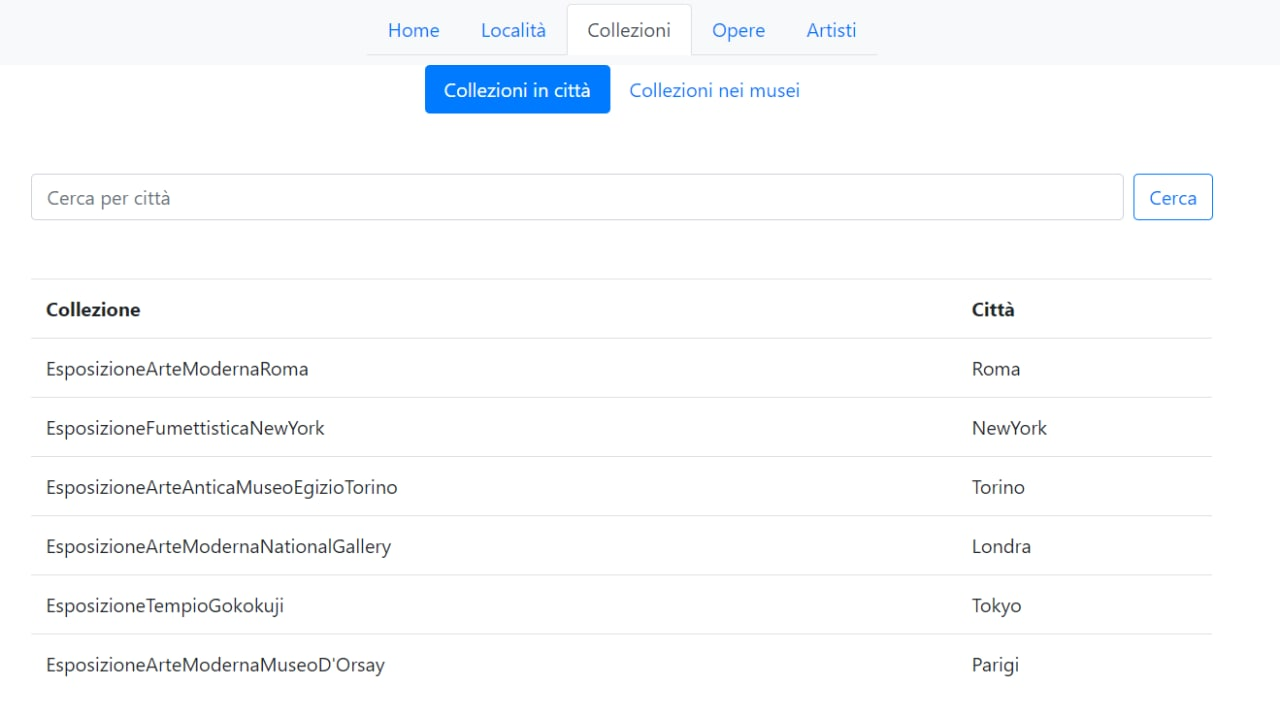
\includegraphics[scale=0.6]{fig/Schermata 3.1 webapp.jpg}
   \caption{Web App - Prima schermata di Collezioni}\label{fig:picture}
      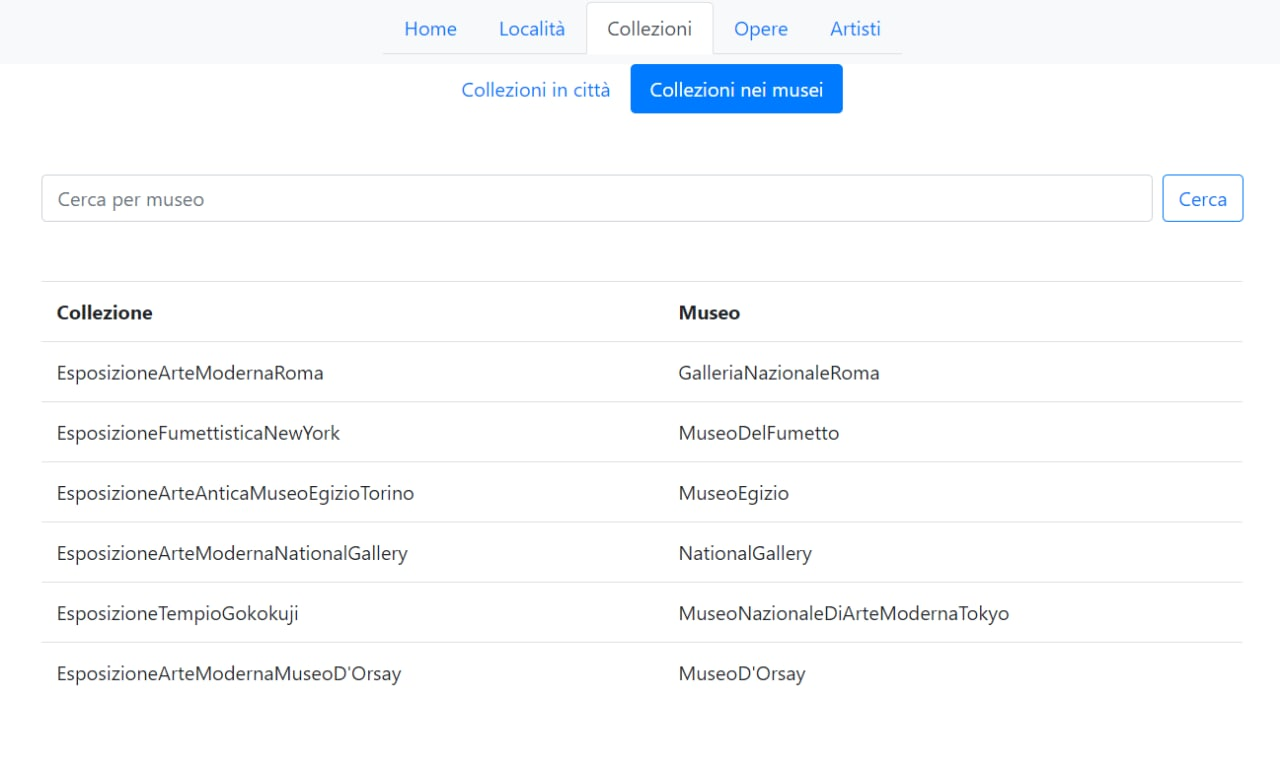
\includegraphics[scale=0.6]{fig/Schermata 3.2 webapp.jpg}
   \caption{Web App - Seconda schermata per Collezioni}\label{fig:picture}
\end{figure}

\newpage
La quarta schermata si focalizza, invece, sulle opere. Più nel dettaglio, l’utente può ricercare un’opera e scoprire la città dove è situata e l’artista che l’ha realizzata. Inoltre, può approfondire la consultazione guardando ai dettagli, quindi all’anno di realizzazione e alla sua descrizione.
Le query in ordine per schermata sono:
\begin{itemize}
 \item SELECT ?opera ?citta ?artista WHERE { ?opera museum:operaInCitta ?citta; museum:realizzatoDa ?artista. FILTER regex(?opera, $<$opera$>$).} ORDER BY ?opera
 \item SELECT ?opera ?artista ?anno ?contenutoDes WHERE{ ?opera museum:realizzatoDa ?artista OPTIONAL {?opera museum:realizzataNel ?anno} OPTIONAL{?opera museum:haDescrizione ?descrizione. ?descrizione museum:contenutoDescrizione ?contenutoDes}  FILTER regex(?opera, $<$opera$>$).}
\end{itemize} 

\begin{figure}[!h]
   \centering
   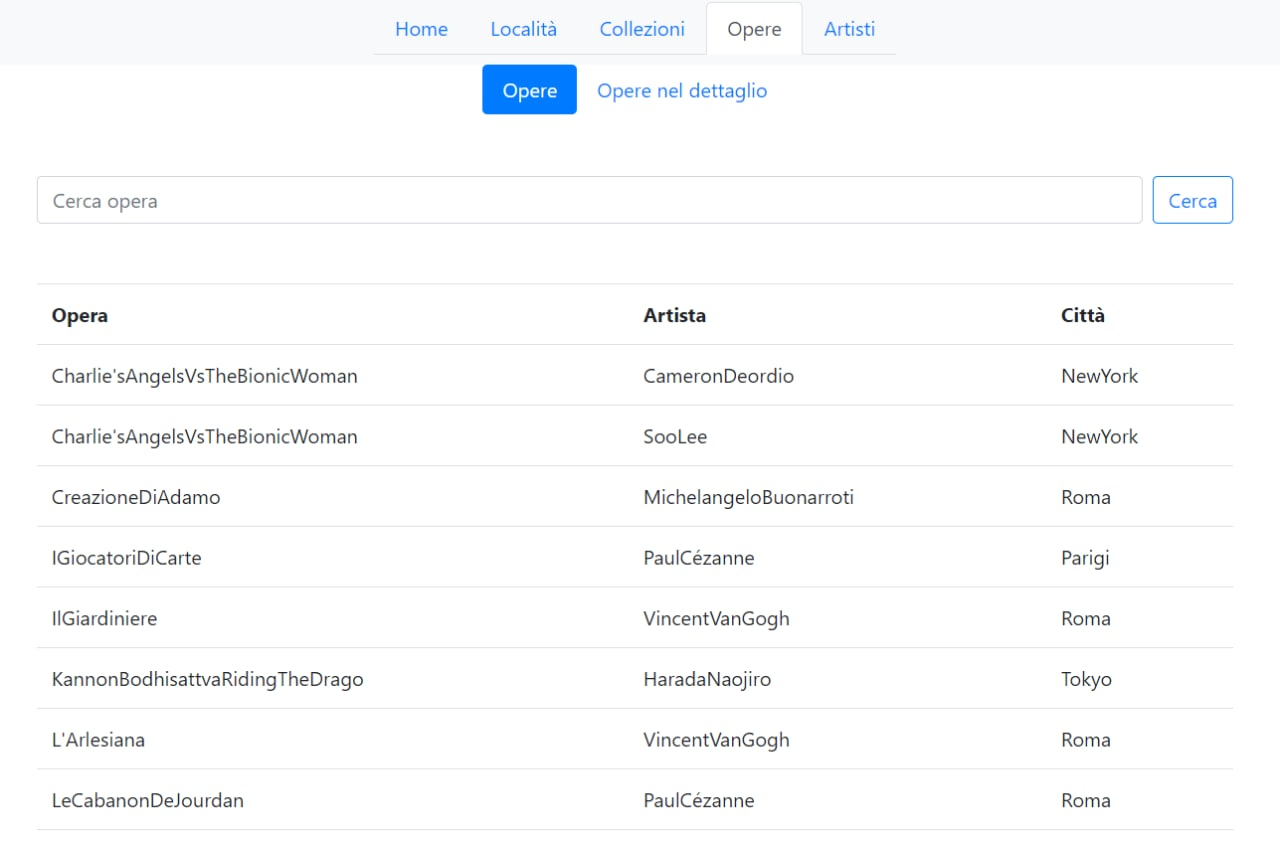
\includegraphics[scale=0.6]{fig/Schermata 4.1 webapp.jpg}
   \caption{Web App - Prima schermata di Opere}\label{fig:picture}
\end{figure}
\begin{figure}[!ht]
   \centering
   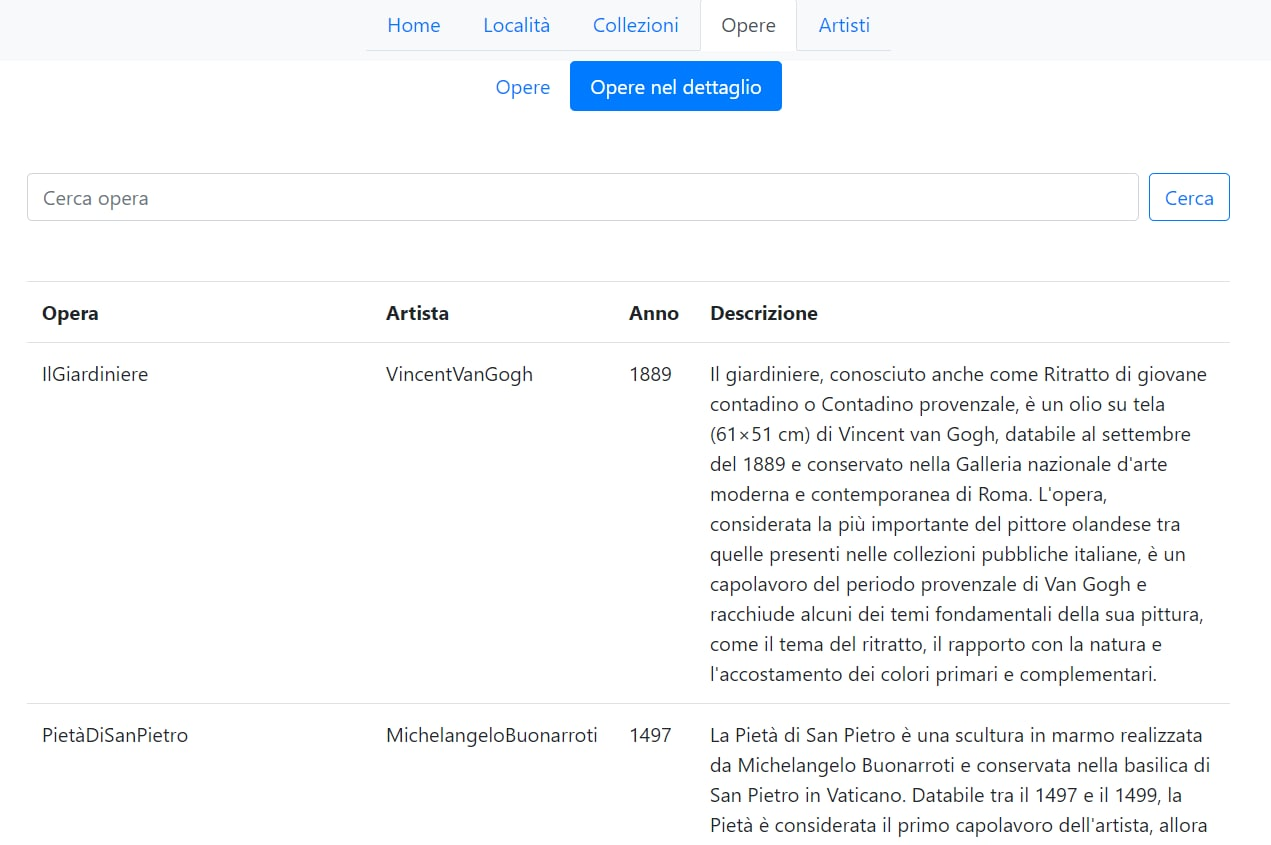
\includegraphics[scale=0.6]{fig/Schermata 4.2 webapp.jpg}
   \caption{Web App - Seconda schermata di Opere}\label{fig:picture}
\end{figure}

\newpage
Le viste dell’ultima schermata danno un ulteriore suggerimento all’utente, ossia gli artisti di cui potrebbe approfondire la ricerca, e riportano dove le opere di questi sono collocate.
Le query in ordine per schermata sono:

\begin{itemize}
 \item SELECT ?artista ?count WHERE{ SELECT ?artista (COUNT(?artista) as ?count) WHERE { ?artista museum:haRealizzato ?opera.} } GROUP BY ?artista HAVING (?count $>$ 1)
 \item SELECT ?artista ?museo ?citta WHERE {?artista museum:presentaIn ?museo. ?museo museum:museoInCitta ?citta. FILTER regex(?artista, $<$artista$>$).} ORDER BY ?artista
\end{itemize} 

Essendo l’ontologia piccola, si è preferito definire grandi artisti coloro i quali abbiano almeno realizzato più di un’opera.\\
Per una visione completa di tutte le query SPARQL formulate si rimanda a questo \href{https://github.com/ModSem20-21/MuseumOntology/blob/master/Query%20SPARQL/Query%20SPARQL.pdf}{link}.

\begin{figure}[!p]
   \centering
   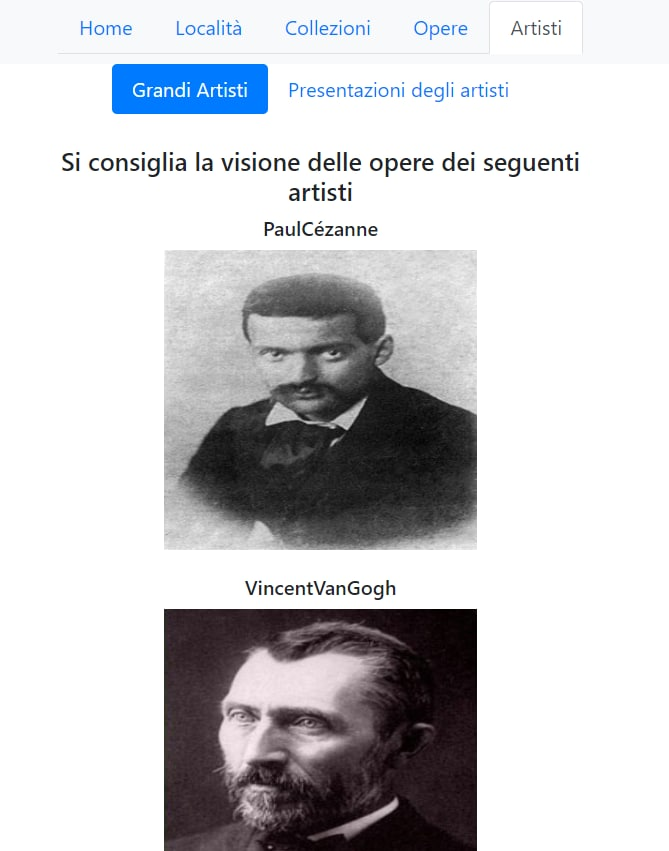
\includegraphics[scale=0.5]{fig/Schermata 5.1 webapp.jpeg}
   \caption{Web App - Prima schermata Artisti}\label{fig:picture}
      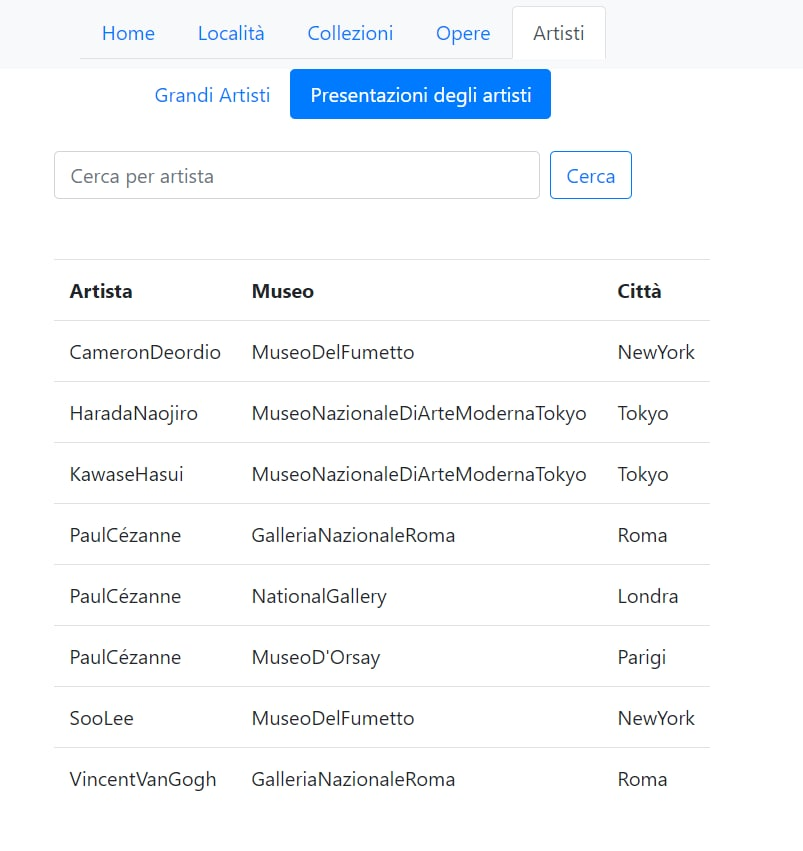
\includegraphics[scale=0.5]{fig/Schermata 5.2 webapp.jpeg}
   \caption{Web App - Seconda schermata Artisti}\label{fig:picture}
\end{figure}
%%%%%%%%%%%%%%%%%%%%%%%%%%%%%%%%%%%%%%%%%%%%%%%%%%%%%%%%%%%%%%%%%%%%
\newpage
\section{Base di regole SWRL}

\begin{itemize}
 \item \textbf{Se un’opera è anche un museo allora fa parte della categoria Museo-Opera:}		
\end{itemize} 
\begin{center}
museum:Museo(?x) \textasciicircum \, museum:Opera(?x) -$>$ museum:MuseoOpera(?x)
\end{center}

\begin{itemize}
 \item \textbf{Se un’opera è stata realizzata dopo il 1800 allora è un’opera moderna:}
\end{itemize} 
\begin{center}
museum:Opera(?x) \textasciicircum \, museum:realizzataNel(?x, ?a) \textasciicircum \, swrlb:greaterThanOrEqual(?a, 1800) \\
-$>$ \\
museum:OperaModerna(?x)
\end{center}

\begin{itemize}
 \item \textbf{Se una collezione è presentata in un museo italiano allora è una collezione italiana:}
\end{itemize} 
\begin{center}
museum:Collezione(?x) \textasciicircum \, museum:presentataIn(?x, ?m) \textasciicircum \\
museum:museoInCitta(?m, ?c) \textasciicircum \, museum:contenutaIn(?c, ?n) \textasciicircum \\
museum:nomeNazione(?n, ?i) \textasciicircum \, swrlb:containsIgnoreCase(?i, "italia") \\
-$>$ \\
museum:CollezioneItaliana(?x)
\end{center}

\begin{itemize}
 \item \textbf{Se una stessa opera è stata realizzata da due artisti diversi allora è un’opera in comune:}
\end{itemize} 
\begin{center}
museum:haRealizzato(?a1, ?o1) \textasciicircum \, museum:haRealizzato(?a2, ?o2) \textasciicircum \\
sameAs(?o1, ?o2) \textasciicircum \, differentFrom(?a1, ?a2) \\
-$>$ \\
museum:OperaInComune(?o1)
\end{center}

\begin{itemize}
 \item \textbf{Allineamento dell’individuo “National Gallery” dell’ontologia sviluppata con quello di DBPedia:}
\end{itemize} 
\begin{center}
museum:nomeMuseo(?m, ?n) \textasciicircum \,
swrlb:containsIgnoreCase(?n, "National Gallery") \\
-$>$ \\
sameAs(?m, autogen0:National\_Gallery)
\end{center}
%%%%%%%%%%%%%%%%%%%%%%%%%%%%%%%%%%%%%%%%%%%%%%%%%%%%%%%%%%%%%%%%%%%%
\newpage
\section{Conclusioni}
Il progetto presentato mostra sicuramente diversi possibili futuri sviluppi. Innanzitutto vi è la possibilità di continuare ad arricchire l'ontologia
aggiungendo istanze di musei, opere e artisti.\\
Inoltre, essendoci diversi standard che riguardano la stessa materia, è possibile fare ulteriori
allineamenti con questi e rendere l'ontologia siffatta più interoperabile. \\
Oltre a ciò, sarebbe interessante sviluppare un sistema più ingegnoso di suggerimenti per gli utenti e per la creazione di itinerari turistici.\\
Riguardo al primo sarebbe necessario introdurre un sistema di profilazione che quindi possa in automatico filtrare le ricerche in base all'utente che sta navigando;
il secondo prevederebbe l'implementazione di una mappa interattiva, magari con l'uso di API esterne come quella di Google Maps, per permettere non solo all'utente
di vedere in tempo reale ad esempio la distanza che intercorre tra sé e il museo che ricerca, ma anche per avere una chiara visualizzazione di un percorso turistico
da comporre.
%%%%%%%%%%%%%%%%%%%%%%%%%%%%%%%%%%%%%%%%%%%%%%%%%%%%%%%%%%%%%%%%%%%%
\newpage
\printbibliography

\end{document}
